\documentclass{beamer}
\usepackage{beamerthemesplit}
% \usepackage{pstricks}
\usepackage{graphicx}
\usepackage{mdwlist}
\usepackage{lineno, hyperref}

\usepackage{amssymb,latexsym,amsmath,amsthm,bbm}
\usepackage{hyperref}
\usepackage{tikz}
\usepackage[english]{babel}
\usepackage[latin1]{inputenc}
\usepackage{multirow}
\usepackage{verbatim}
\usepackage{alltt}
\usepackage{mycommands}

\usepackage{cmbright}
\renewcommand*\familydefault{\sfdefault}
\usepackage[T1]{fontenc}


\definecolor{wp-red}{RGB}{204,0,0}
\definecolor{wp-gray}{RGB}{51,51,51}
\definecolor{reynolds-red}{RGB}{153,0,0}
\definecolor{pyroman-flame}{RGB}{209,81,34}
\definecolor{hunt-yellow}{RGB}{253,215,38}
\definecolor{genomic-green}{RGB}{125,140,31}
\definecolor{innovation-blue}{RGB}{66,126,147}
\definecolor{bio-indigo}{RGB}{65,86,161}

\setbeamercolor{structure}{fg=wp-red}
\setbeamercolor{title}{bg=white, fg=wp-red}  % changes color on title page
\setbeamerfont{title}{series=\bfseries, size=\huge}
\setbeamerfont{author}{series=\bfseries, size=\large}
\setbeamerfont{institute}{series=\mdseries, size=\large}

\setbeamercolor{frametitle}{bg=wp-red, fg=white}  % changes color at top of frame
\setbeamerfont{frametitle}{series=\bfseries}
\setbeamercolor{title in head/foot}{fg=white, bg=wp-red}  % changes color for title in footer
\setbeamerfont{title in head/foot}{series=\bfseries}
\setbeamercolor{author in head/foot}{fg=white,bg=wp-gray}  % changes color for author in footer
\setbeamerfont{author in head/foot}{series=\bfseries}


\title[Spatiotemporal Modeling of Extreme Events] % (optional, use only with long paper titles)
{
  Spatiotemporal Modeling of Extreme Events
}
\author[S. Morris, B. Reich, and D. Cooley]{Samuel Morris (NC State), Brian Reich (NC State), and Dan Cooley (Colorado State)}
\institute[NCSU, CSU]{}
\date{JSM 2014, Boston}

\begin{document}

\begin{frame}\frametitle{\ }
\begin{center}
	\maketitle
\end{center}
\end{frame}

\begin{frame}{Motivation}
  \begin{itemize} \setlength{\itemsep}{1em}
    \item Average behavior is important to understand, but it does not paint the whole picture
    \begin{itemize}
      \item e.g. When constructing river levees, engineers need to be able to estimate a 100-year or 1000-year flood levels
      \item e.g. Probability of exceeding a certain threshold level
    \end{itemize}
    \item Spatial methods borrow information across space to estimate spatial correlation and make predictions by Kriging at unknown locations
    \item Want to explore similar methods for extremes
  \end{itemize}
\end{frame}

% \begin{frame}{Introduction to extremes}
%   \begin{itemize} \setlength{\itemsep}{0.5em}
%     \item Max-stable processes (Cooley et al., 2012):
%     \begin{itemize}
%       \item Consider a spatial process $x_t(\bs)$, $t = 1, \ldots, T$.
%       \item Let $M_T(\bs) = \left\{ \bigvee_{t=1}^T x_t(\bs_1), \ldots, \bigvee_{t=1}^T x_t(\bs_n) \right\}$
%       \item If there exists normalizing sequences $a_T(\bs)$ and $b_T(\bs)$ such
%       that for all sites, $\bs_i, i = 1, \ldots, d$,
%       \begin{align*}
%         a_T^{-1}(\bs) \left\{ M_T(\bs) - b_T(\bs) \right\} \converged Y(\bs)
%       \end{align*}
%       which has a non-degenerate distribution, then $Y(\bs)$ is a max-stable process.
%     \end{itemize}
%   \end{itemize}
% \end{frame}

\begin{frame}{Standard analysis - Block maxima}
  \begin{itemize} \setlength{\itemsep}{0.5em}
      \item Uses yearly maxima
      \item Discards many observations
      \item Models are fit using the generalized extreme value distribution
    \item For a spatial analysis, max-stable processes give an appropriate limiting distribution
  \end{itemize}
\end{frame}

\begin{frame}{Standard analysis - Peaks over threshold}
  \begin{itemize}  \setlength{\itemsep}{0.5em}
      \item Incorporates more data than block maxima
      \item Select a threshold, $T$, and use the Generalized Pareto distribution (GPD) to model the exceedances
      \item Temporal dependence may be an issue between observations (e.g. flood levels don't dissipate overnight)
  \end{itemize}
\end{frame}

% \begin{frame}{Multivariate representations}
%   \begin{itemize}
%     \item Multivariate distributions:
%     \begin{itemize}
%       \item Assume common standardized max-stable marginal, like unit-Fr\'{e}chet
%       \begin{align*}
%         \Pr(Z < z) = exp(-z^{-1})
%       \end{align*}
%       \item The multivariate representation for the GEV is
%       \begin{align*}
%         \Pr(\bZ \le \bz)  &= G^*(\bz) = \exp(-V(\bz))\\
%                 V(\bs)    &= d \int_{\Delta_d} \bigvee_{i = 1}^d \frac{w_i}{z_i} H(\ddd w)
%       \end{align*}
%       where
%       \begin{itemize}
%         \item $\Delta_d = \{ \bw \in \calR^d_+ \mid w_1 + \cdots + w_d = 1\}$
%         \item $H$ is a probability measure on $\Delta_d$
%         \item $\int_{\Delta_d}w_i H(\ddd w) = 1 / d$ for $i = 1, \ldots, d$.
%       \end{itemize}
%     \end{itemize}
%   \end{itemize}
% \end{frame}

\begin{frame}{Multivariate analysis}
  \begin{itemize} \setlength{\itemsep}{0.5em}
    \item Multivariate max-stable and GPD models have nice features, but they are
    \begin{itemize}
      \item computationally challenging to work with
      \item joint distribution only available in low dimension
    \end{itemize}
    \item Pairwise likelihood approach (Huser and Davison, 2014)
  \end{itemize}
\end{frame}

\begin{frame}{Model objectives}
  \begin{itemize} \setlength{\itemsep}{0.5em}
    \item Our objective is to build a model that
    \begin{itemize}
      \item has marginal distribution with a flexible tail
      \item has asymptotic spatial dependence
      \item has computation on the order of Gaussian models for large space-time datasets
    \end{itemize}
  \end{itemize}
\end{frame}

\begin{frame}{Thresholding data}
  \begin{itemize} \setlength{\itemsep}{0.5em}
    \item We threshold the observed data at a high threshold $T$.
    \item Thresholded data:
    \begin{align*}
      Y_t^*(\bs) = \left\{ \begin{array}{ll}
          Y_t(\bs) \quad & Y_t(\bs) > T\\
          T \quad & Y_t(\bs) \le T
      \end{array}\right.
    \end{align*}
    \item Allows tails of the distribution to speak for themselves.
  \end{itemize}
\end{frame}

\begin{frame}{$\chi$ coefficient}
  \begin{itemize} \setlength{\itemsep}{0.5em}
   \item The $\chi$ coefficient is a measure of extremal dependence
   \item Specifically, we focus on $\chi(\bh)$ for the upper tail given by
    \begin{align*}
      \chi(\bh) = \lim_{c \rightarrow \infty}\Pr(Y(\bs) > c \mid Y(\bs + \bh) > c)
    \end{align*}
    \item If $ \chi(\bh) = 0$, then observations are asymptotically independent at distance $\bh$.
    \item We expect $\lim_{\bh \rightarrow \infty}\chi(\bh)=0$.
  \end{itemize}
\end{frame}

\begin{frame}{Gaussian spatial model}
  \begin{itemize} \setlength{\itemsep}{0.5em}
    \item In geostatistics $Y(\bs)$ are often modeled using a Gaussian process with mean function $\mu(\bs)$ and covariance function
$\rho(\bh)$.
    \item Model properties:
    \begin{itemize}
      \item Nice computing properties (closed-form likelihood)
    \item For a Gaussian spatial model $\lim_{c \rightarrow \infty} \chi(\bh) = 0$ regardless of the strength of the correlation in the bulk of the distribution
    \item Tail is not flexible (Gaussian is light tailed)
    \end{itemize}
    \end{itemize}
\end{frame}

\begin{frame}{Spatial skew-$t$ distribution}
  \begin{itemize} \setlength{\itemsep}{0.5em}
    \item Assume observed data $Y_t(\bs)$ come from a skew-$t$ (Zhang and El-Shaarawi, 2012)
    \begin{align*}
      Y_t(\bs) = X_t(\bs)\beta + \alpha z_t + v_t(\bs)
    \end{align*}
    where
    \begin{itemize} \setlength{\itemsep}{0.25em}
      \item $\alpha \in \calR$ controls the skewness
      \item $z_t \iid N_{(0, \infty)}(0, \sigma^2_t)$ is a random effect
      \item $v_t(\bs)$ is a Gaussian process with variance $\sigma^2_t$ and \Matern correlation
      \item $\sigma_t^2 \iid \text{IG}(a, b)$
    \end{itemize}
  \end{itemize}
\end{frame}

\begin{frame}{Spatial skew-$t$ distribution}
  \begin{itemize} \setlength{\itemsep}{0.5em}
   \item \alert{Conditioned} on $z_t$ and $\sigma^2_t$, $Y_t(\bs)$ is a Gaussian spatial model
    \item Can use standard geostatistical methods to fit this model
    \item Predictions can be made through Kriging
    \item \alert{Marginalizing} over $z_t$ and $\sigma^2_t$ (via MCMC),
    \begin{align*}
      Y_t(\bs) \sim \text{skew-t}(\mu, \Sigma^*, \alpha, \text{df}=2a)
    \end{align*}
    where
    \begin{itemize}
    	\item $\mu$ is the location
	\item $a$, $b$ are the IG parameters for $\sigma^2_t$
	\item $\Sigma^* = \frac{ b }{ a } \Sigma$ is a scale matrix, and $\Sigma$ is a \Matern covariance matrix
	\item $\alpha \in \calR$ controls the skewness
    \end{itemize}
  \end{itemize}
\end{frame}

\begin{frame}{Spatial skew-$t$ distribution}
  \begin{itemize} \setlength{\itemsep}{0.5em}
      \item Model properties
    \begin{itemize}
    	\item Has flexible tail controlled by skewness $\alpha$ and degrees of freedom $2a$
    	\item For a skew-$t$ distribution $\lim_{c \rightarrow \infty} \chi(\bh) > 0$ (Padoan, 2011)
    	\item Computation that is on the order of Gaussian computation
    \end{itemize}
    \item For this distribution, $\chi(\bh)$ shows asymptotic dependence that does not approach 0 as $\bh \rightarrow \infty$
   \item This occurs because all observations (near and far) share the same $z_t$ and $\sigma_t^2$
    \item We deal with this through a daily random partition (similar to Huser and Davison)
  \end{itemize}
\end{frame}

\begin{frame}{Daily random partition}
  \begin{itemize} \setlength{\itemsep}{0.5em}
    \item Daily random partition allows $z_t$ and $\sigma^2_t$ to vary by site
    \begin{align*}
      Y_t(\bs) = X_t(\bs) \beta + \alpha z_t(\bs) + \sigma(\bs) v_t(\bs)
    \end{align*}
    \item Consider a set of daily knots $\bw_{tk} \sim$ Uniform that define a random daily partition
    $P_{t1}, \ldots, P_{tK}$ such that
    \begin{align*}
      P_{tk} = \{s : k = \argmin_\ell|| \bs - \bw_{t\ell}|| \}
    \end{align*}
    \item For $\bs \in P_{tk}$
    \begin{align*}
      z_t(\bs) &= z_{tk}\\
      \sigma^2_t(\bs) &= \sigma^2_{tk}
    \end{align*}
    \item Within each partition $Y_t(\bs)$ has the same MV skew-t distribution as before
  \end{itemize}
\end{frame}

\begin{frame}{Example daily partition}
    \centering
    \begin{figure}
    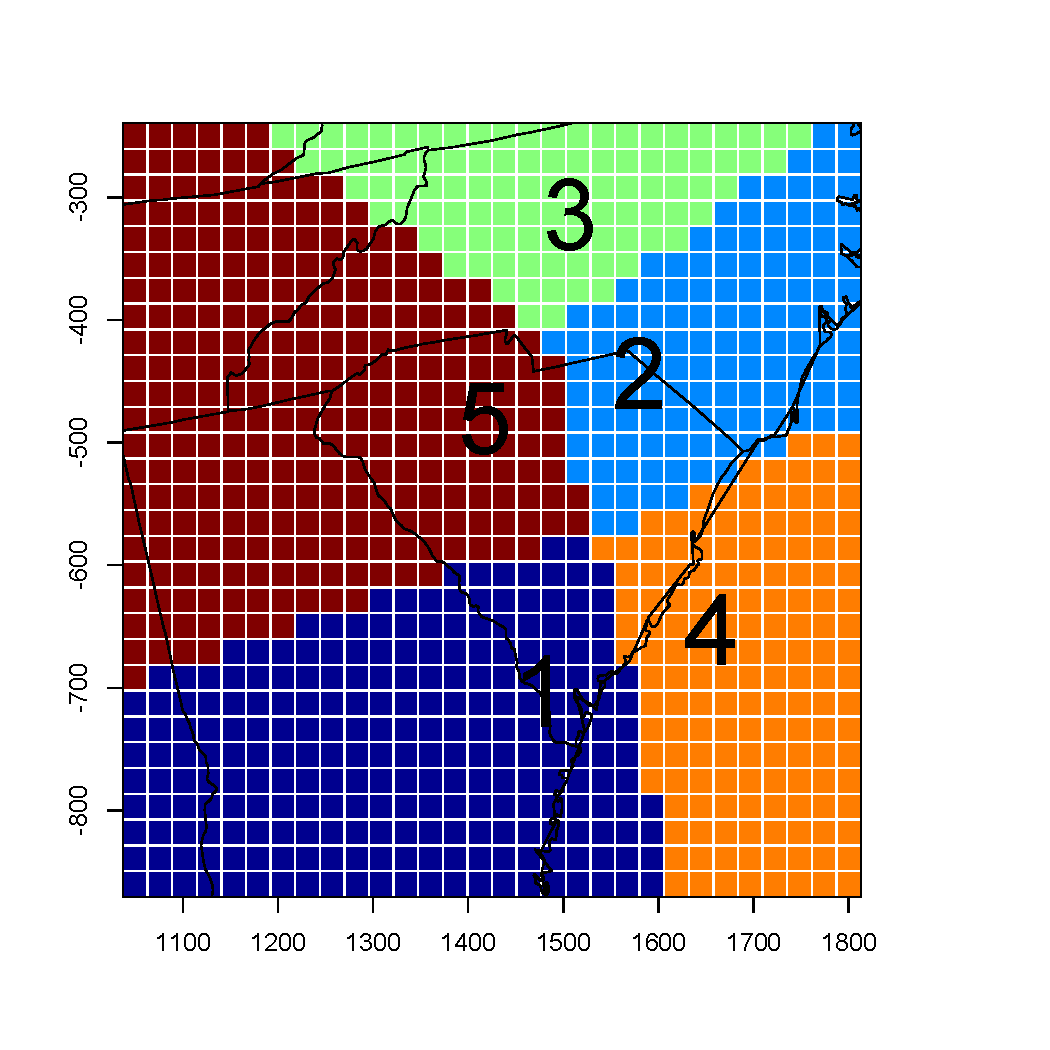
\includegraphics[width=0.54\linewidth]{./plots/example-partition-1.pdf}
    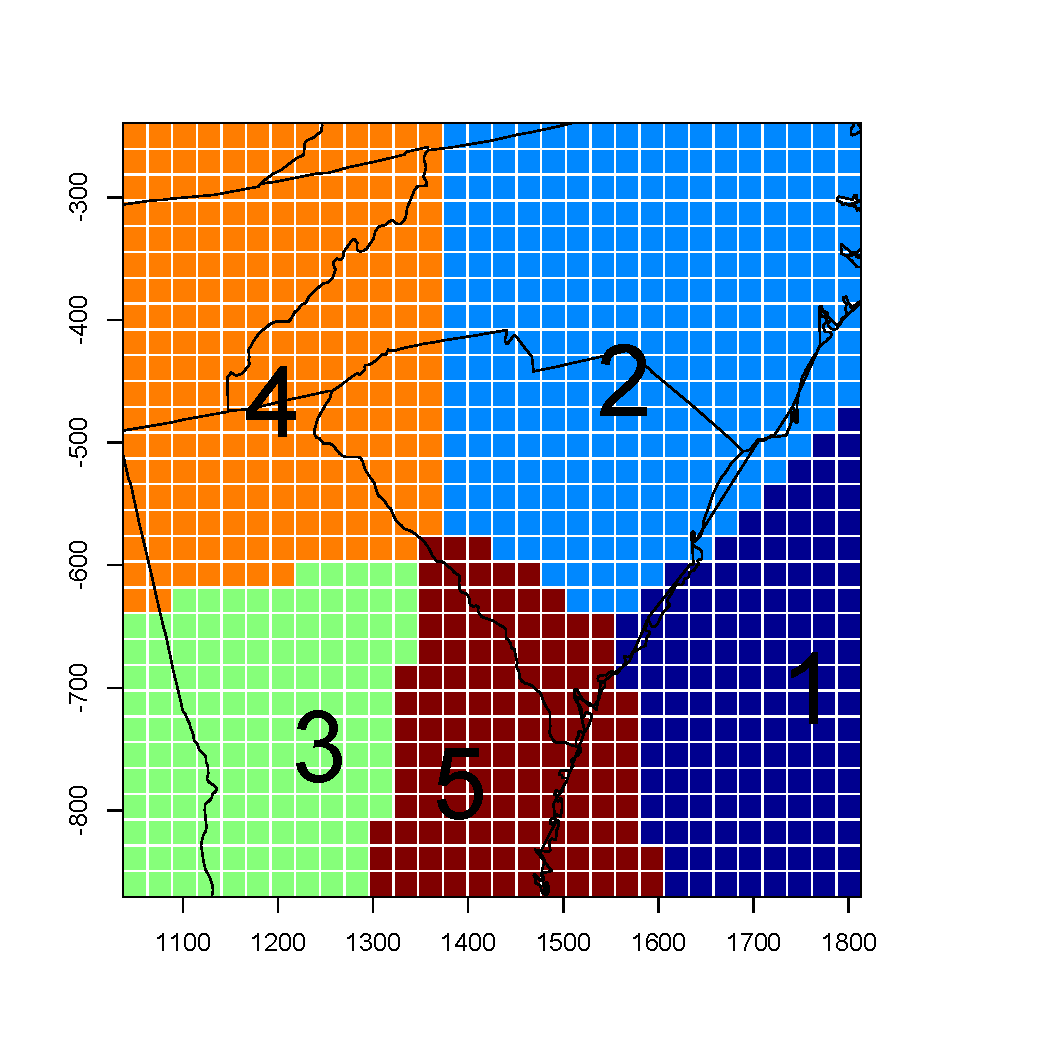
\includegraphics[width=0.54\linewidth]{./plots/example-partition-2.pdf}
    \caption{Two sample partitions (number is at partition center)}
    \end{figure}
\end{frame}


\begin{frame}{Simulated $\widehat{\chi}(\bh)$ plots}
  \centering
  \begin{figure}
  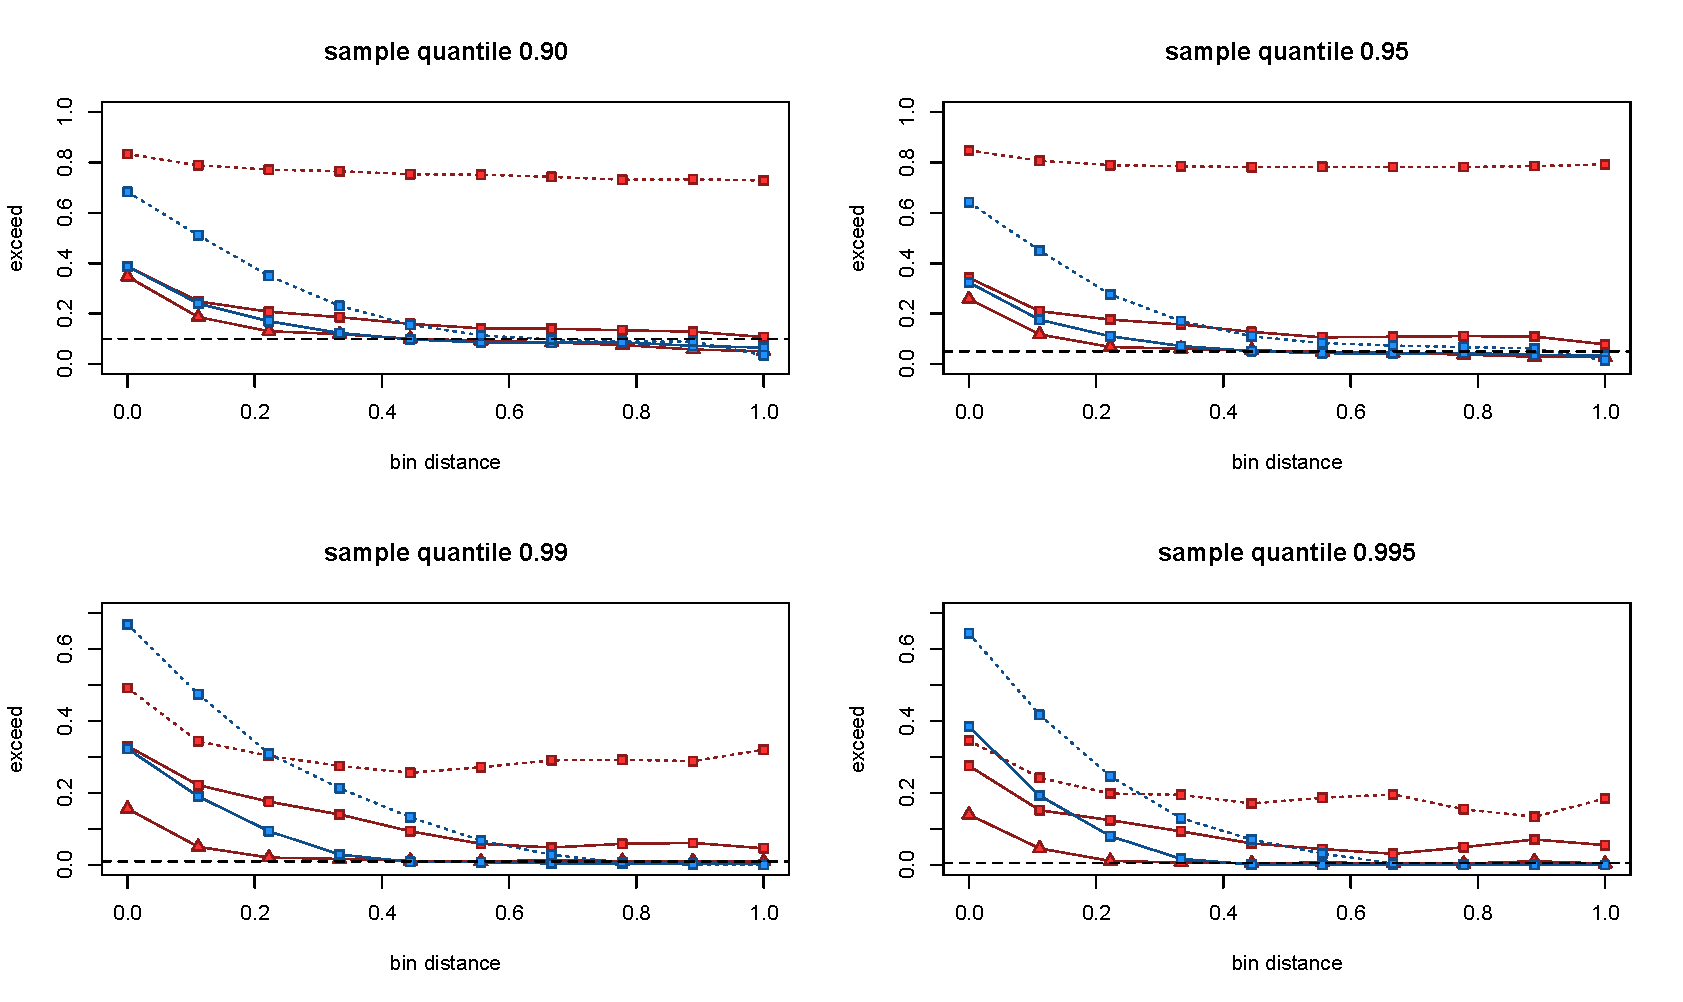
\includegraphics[width=1\linewidth]{./plots/chi-plots.pdf}\\[-0.25in]
  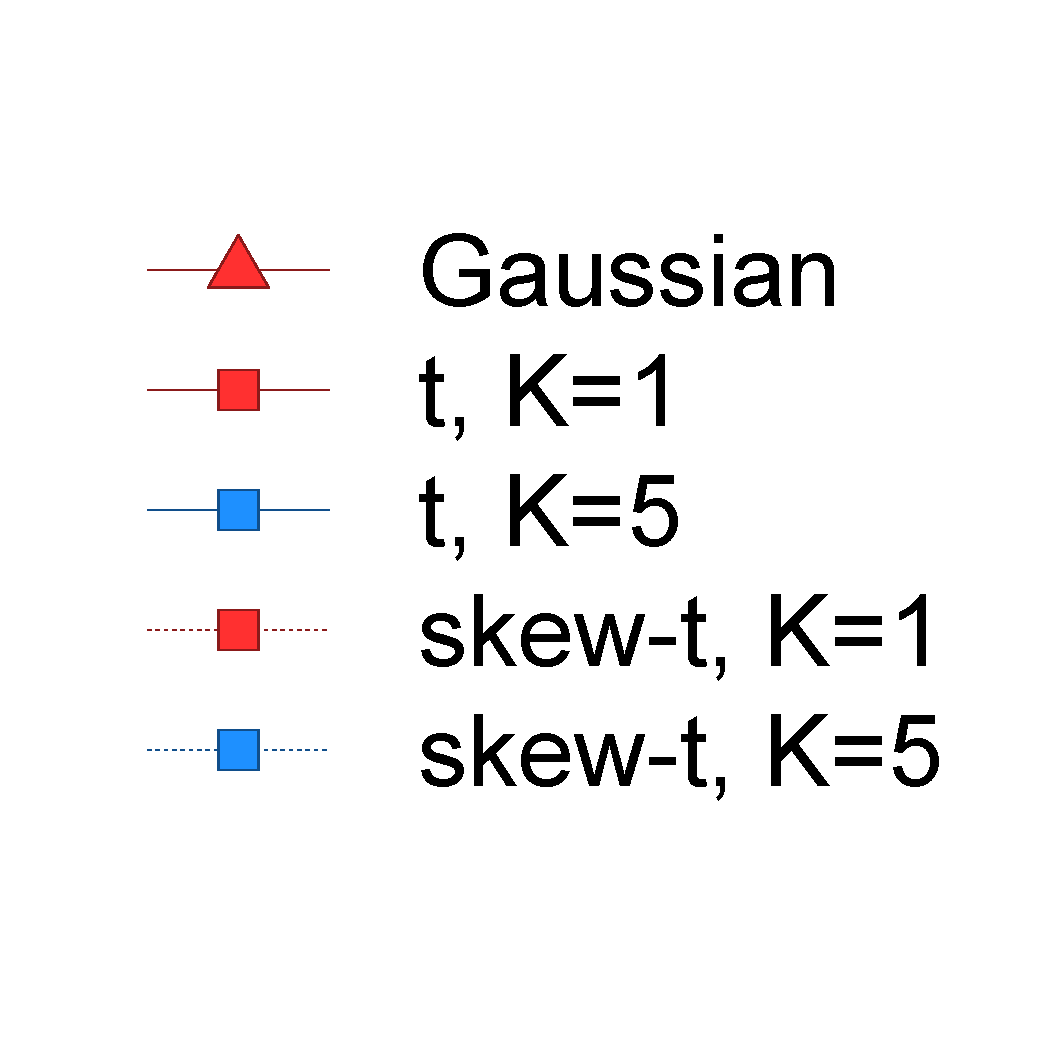
\includegraphics[width=0.2\linewidth]{./plots/chi-legend.pdf}
  \caption{$\chi$ plots from simulated datasets}
  \end{figure}
\end{frame}

\begin{frame}{Sample simulated datasets}
  \centering
  \begin{figure}
  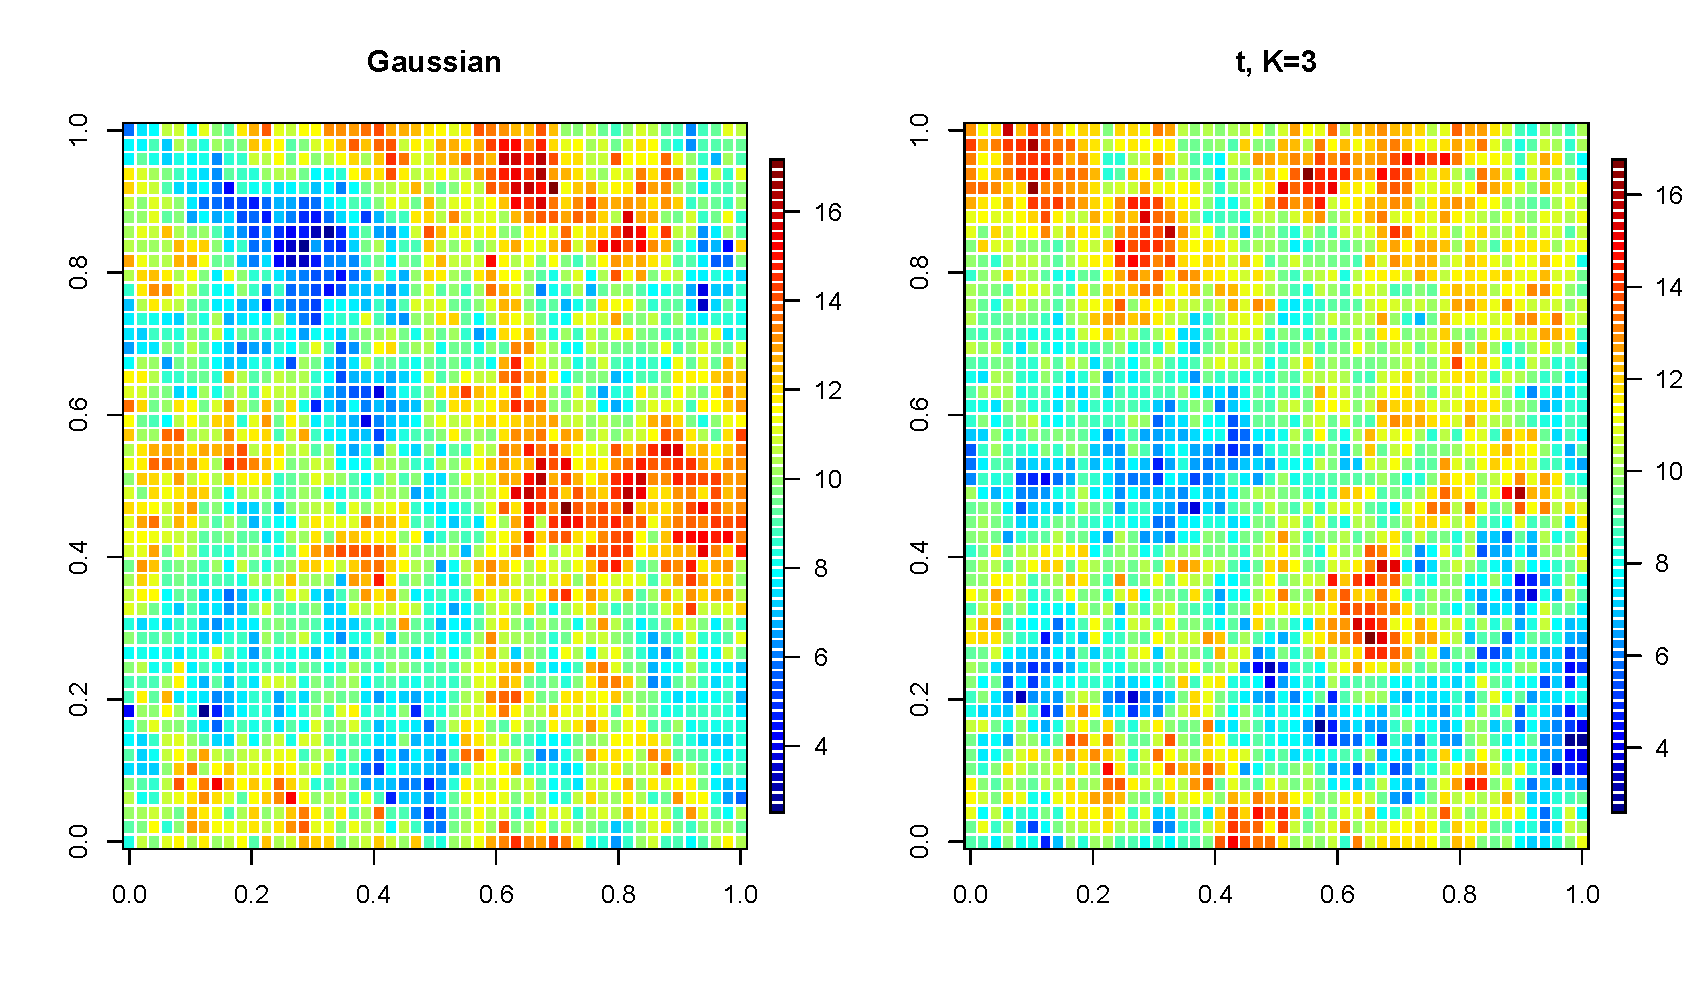
\includegraphics[width=1\linewidth]{./plots/gauss-vs-t3.pdf}
  \caption{Gaussian and $t$ with 3 partitions}
  \end{figure}
\end{frame}

\begin{frame}{Sample simulated datasets}
  \centering
  \begin{figure}
  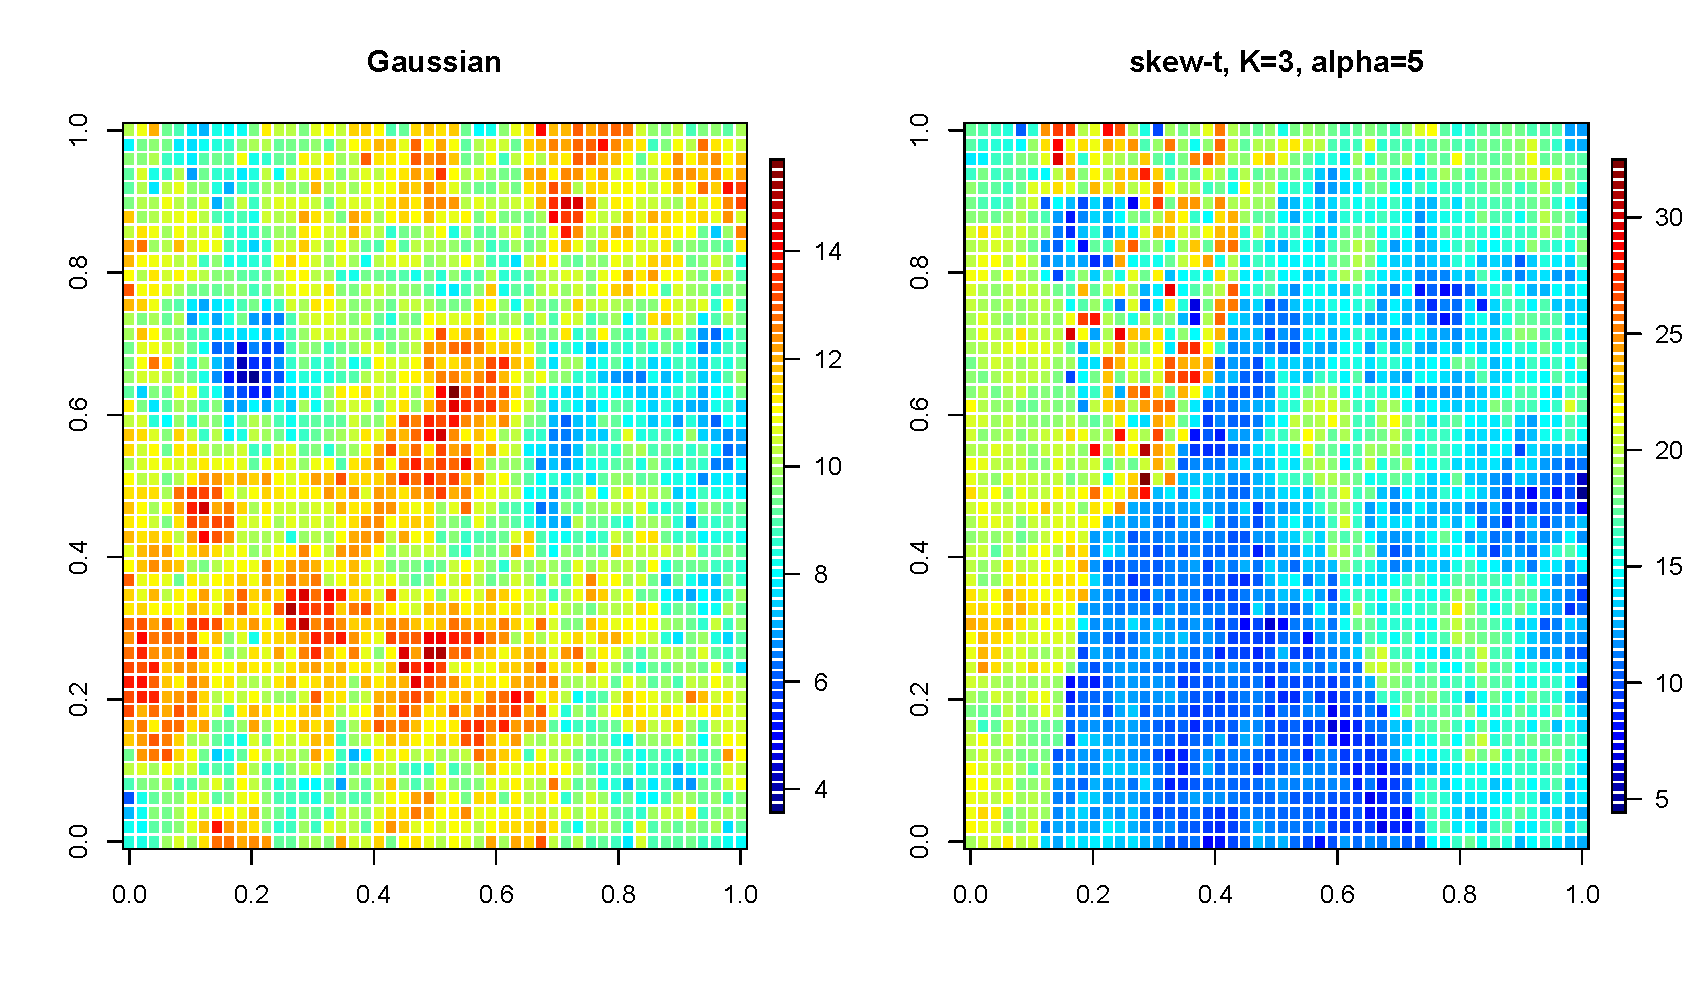
\includegraphics[width=1\linewidth]{./plots/gauss-vs-skew-t3.pdf}
  \caption{Gaussian and skew-$t$ with 3 partitions}
  \end{figure}
\end{frame}

\begin{frame}{MCMC details}
  \begin{itemize} \setlength{\itemsep}{0.5em}
    \item Three main steps:
    \begin{enumerate}[1.]
      \item Impute censored data below $T$
      \item Update parameters with standard random walk Metropolis Hastings or Gibbs sampling
      \item Make spatial predictions
    \end{enumerate}
    \item Priors are selected to be conjugate when possible
  \end{itemize}
\end{frame}

\begin{frame}{Data analysis}
\begin{columns}[c]
\column{.45 \linewidth}
	\begin{itemize} \setlength{\itemsep}{0.5em}
	\item Data analysis uses
	\begin{itemize}
		\item max 8-hour ozone measurements
		\item 85 sites
		\item 92 days
	\end{itemize}
	\end{itemize}
	
	\column{.55\linewidth}
	\begin{figure}
    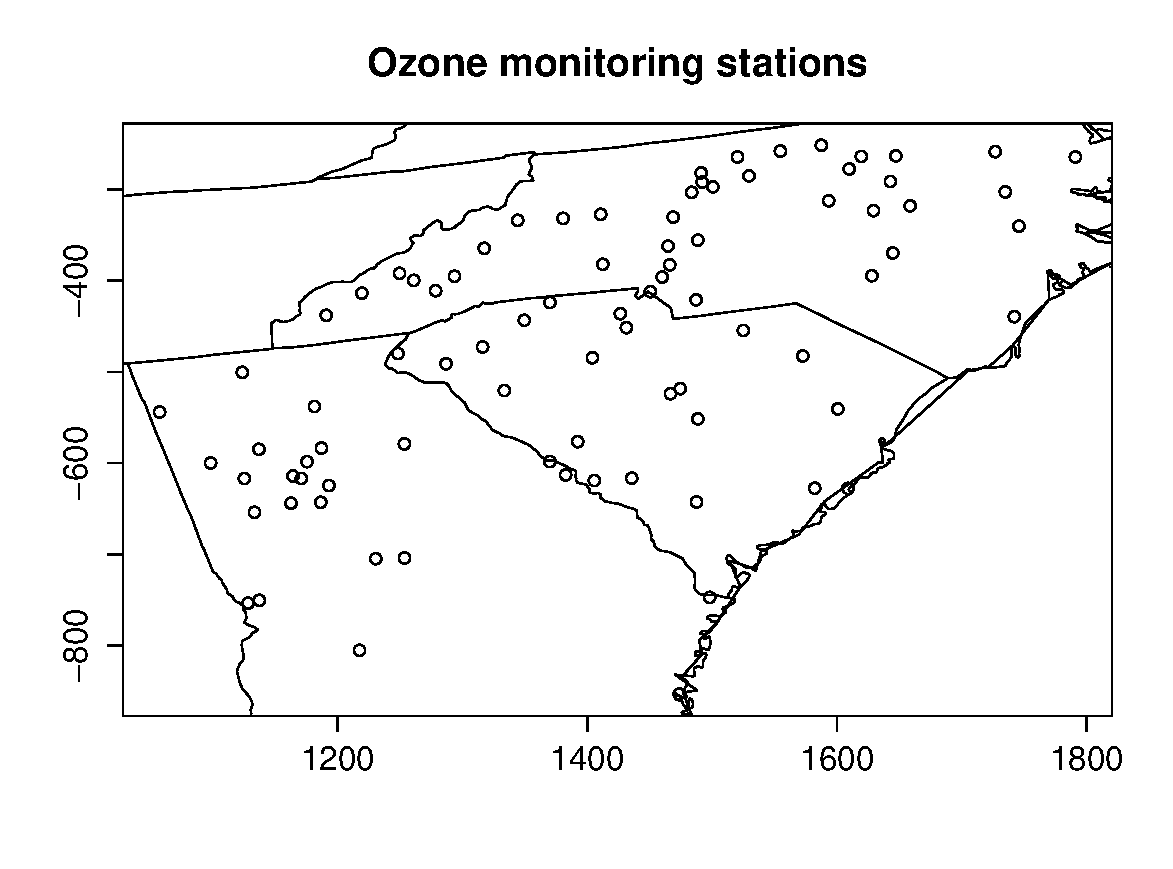
\includegraphics[width=1\linewidth]{./plots/ozone_station.pdf}
    \caption{Ozone monitoring station locations}
    \end{figure}
\end{columns}
\end{frame}

\begin{frame}{Data analysis}
  \centering
  \begin{figure}
    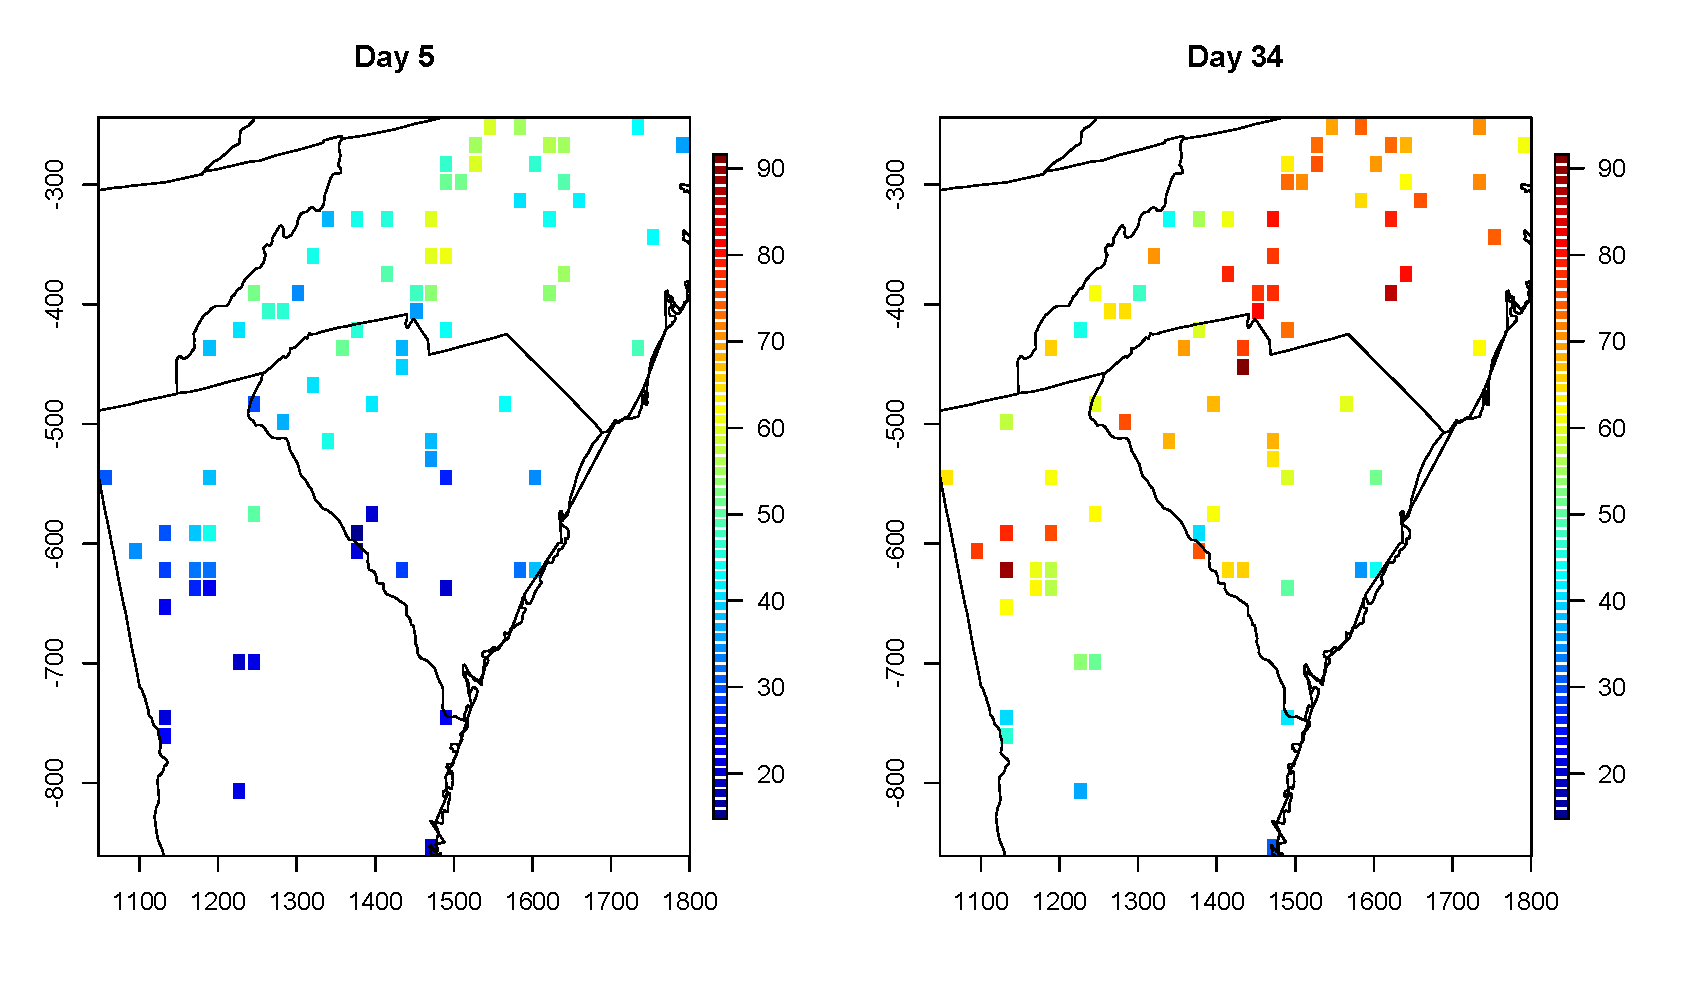
\includegraphics[width=1\linewidth]{./plots/ozone-day.pdf}
    \caption{Max 8-hour ozone measurements at 85 sites in NC, SC, and GA for days 5 and 34}
   \end{figure}

\end{frame}

\begin{frame}{Exploratory data analysis}
	\centering
  \begin{figure}
    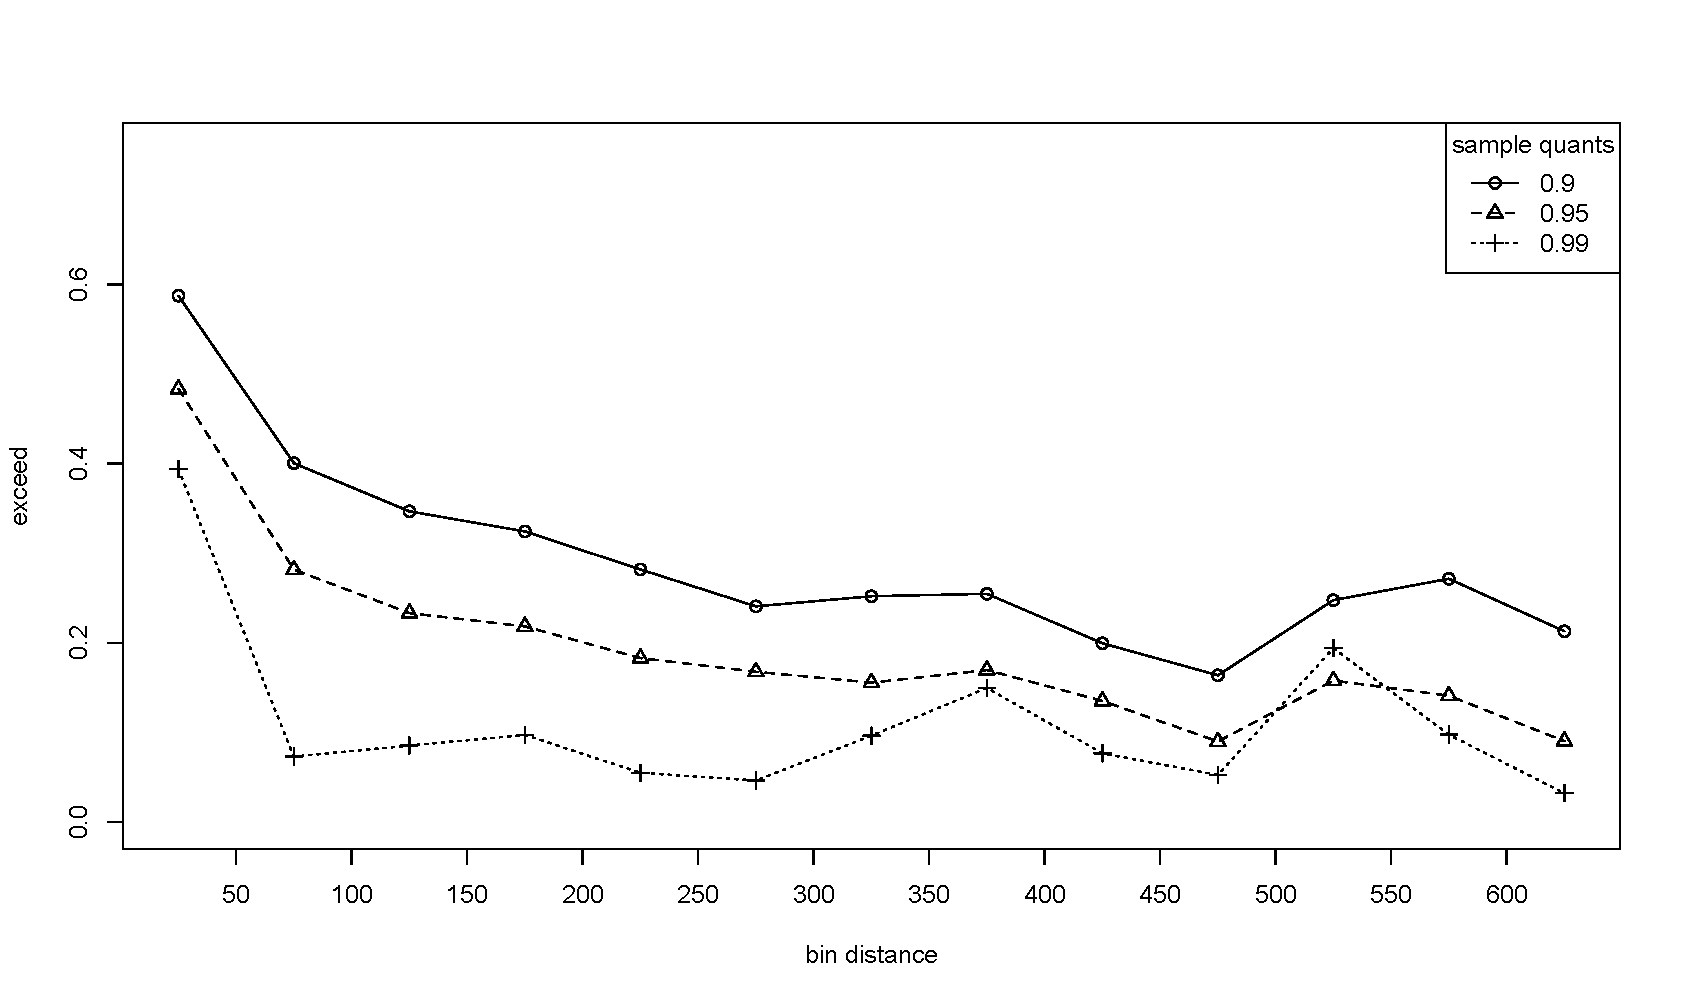
\includegraphics[width=1\linewidth]{./plots/chi-plot-ozone-res.pdf}
    \caption{$\widehat{\chi}$-plot for sample quantiles of ozone observations}
  \end{figure}
\end{frame}

\begin{frame}{Model comparisons}
  \begin{itemize} \setlength{\itemsep}{0.5em}
    \item 9 different analysis methods incorporating
    \begin{itemize}
      \item Gaussian vs $t$ vs skew-$t$ marginal distribution
      \item $K=1$ partition vs $K=3$ partitions
      \item No thresholding vs thresholding at $T=0.90$ sample quantile
    \end{itemize}
    \item All methods use a \Matern or exponential covariance ($\nu = 0.5$)
    \item Compare quantile and Brier scores using 5-fold cross validation (Gneiting and Raftery, 2007)
    \item Mean function modeled as
    \begin{align*}
    	\beta_0 + \beta_1 \cdot \text{lat} + \beta_2 \cdot \text{long} +  \beta_3 \cdot \text{lat}^2 + \beta_4 \cdot \text{long}^2 + \beta_5 \cdot \text{lat} \cdot \text{long} 
    \end{align*}
   \end{itemize}
\end{frame}

\begin{frame}{Quantile score for cross-validation}
  \begin{itemize} \setlength{\itemsep}{0.5em}
    \item The quantile score for the $\tau$th quantile is
    \begin{align*}
      2 \{ I[y < \widehat{q}(\tau)] - \tau\} (\widehat{q} - y)
    \end{align*}
    where:
    \begin{itemize}
      \item $y$ is a test set value
      \item $\widehat{q}(\tau)$ is the estimated $\tau$th quantile
    \end{itemize}
  \end{itemize}
\end{frame}

\begin{frame}{Brier score}
  \begin{itemize} \setlength{\itemsep}{0.5em}
	\item The Brier score for predicting exceedance of threshold $c$ is
	\begin{align*}
	  [e(c) - P(c)]^2
	\end{align*}
	where
	\begin{itemize}
		\item $y$ is a test set value
		\item $e(c) = I[y > c]$
		\item $P(c)$ is the predicted probability of exceeding $c$
	\end{itemize}
  \end{itemize}
\end{frame}

\begin{frame}{Five-fold cross-validation results}
  \begin{table}[htbp]
    \small
    \centering
    \begin{tabular}{l|c|r|rrrrr}
          \multicolumn{3}{c}{\ } & \multicolumn{5}{c}{$\tau$}\\
           \hline
  Marginal & $K$ & $T$  & 0.950 & 0.980 & 0.990 & 0.995 & 0.999\\
  \hline
Gaussian 	& 1 & 0 	& 39.820 & 17.539 & 9.167 & 4.720 & 1.057\\
$t$		& 1 & 0 	& {\bf 31.008} & {\bf 13.898} & 7.229 & {\bf 3.405} & 0.879\\
$t$		& 3 & 0	& 31.213 & 13.920 & {\bf 7.218} & 3.498 & 0.918\\
$t$		& 1 & 0.9	& 32.221 & 14.519 & 7.549 & 3.604 & 0.896\\
$t$		& 3 & 0.9 	& 38.842 & 16.781 & 8.434 & 4.180 & 1.020\\
skew-$t$	& 1 & 0	& 31.845 & 14.542 & 7.533 & 3.645 & {\bf 0.844}\\
skew-$t$	& 1 & 0.9	& 32.132 & 14.296 & 7.484 & 3.497 & 0.890\\
skew-$t$	& 3 & 0	& 33.653 & 15.453 & 8.119 & 4.338 & 1.188\\
skew-$t$	& 3 & 0.9 	& 32.157 & 14.727 & 7.794 & 3.825 & 0.917\\
\hline
    \end{tabular}
    \caption{Brier score for predicting exceedance of $c = \hat{q}(\tau)$ from five-fold cross-validation ($\times 1000$)}
  \end{table} \vspace{-1.5em}
  \begin{itemize}
  	\item Quantile score results are similar
  \end{itemize}
\end{frame}

\begin{frame}{Predicted 95th quantile}
\centering
\begin{figure}
    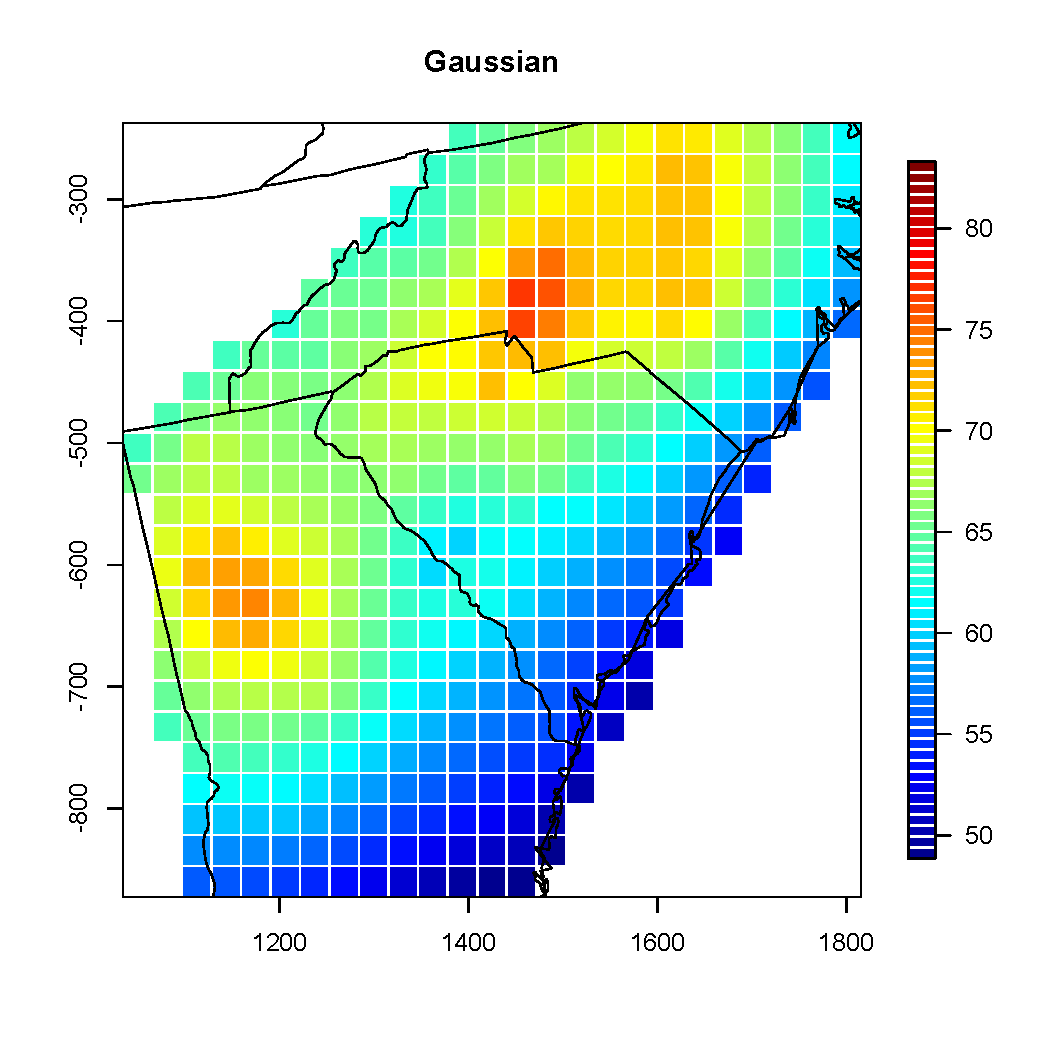
\includegraphics[width=.5\linewidth]{./plots/quantile-95-gau.pdf}
    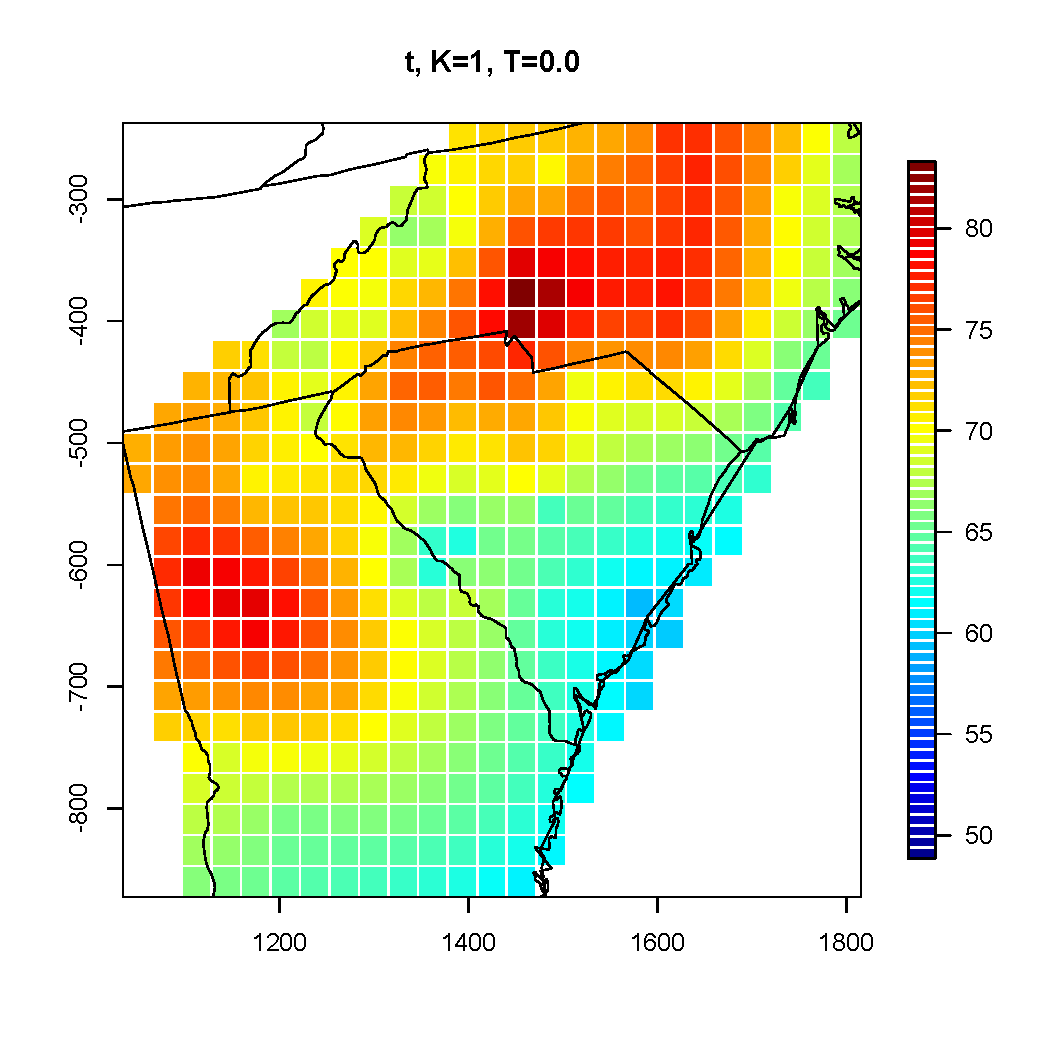
\includegraphics[width=.5\linewidth]{./plots/quantile-95-t10.pdf}
    \caption{Predicted 95th quantile using Gaussian and $t$}
\end{figure}
\end{frame}

\begin{frame}{Predicted 95th quantile}
\centering
\begin{figure}
    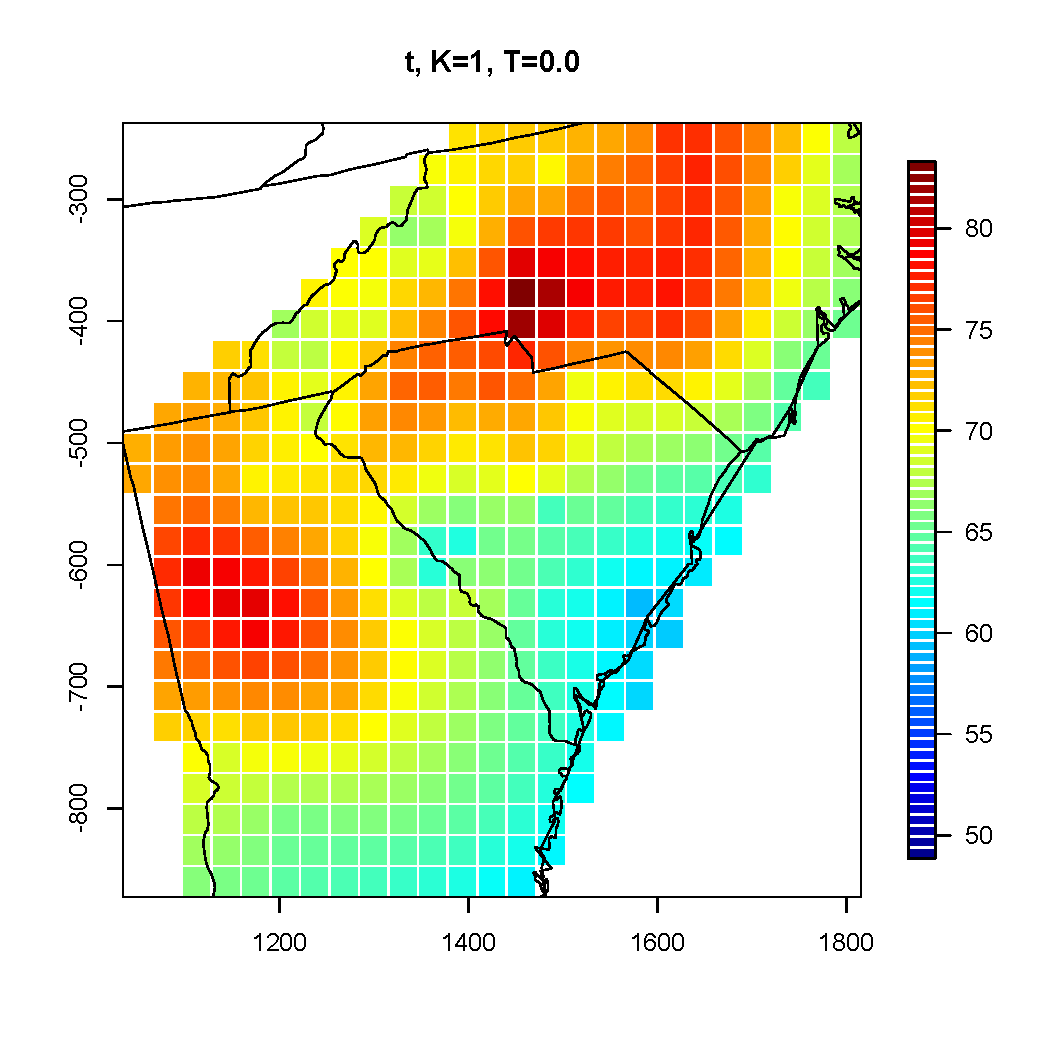
\includegraphics[width=.5\linewidth]{./plots/quantile-95-t10.pdf}
    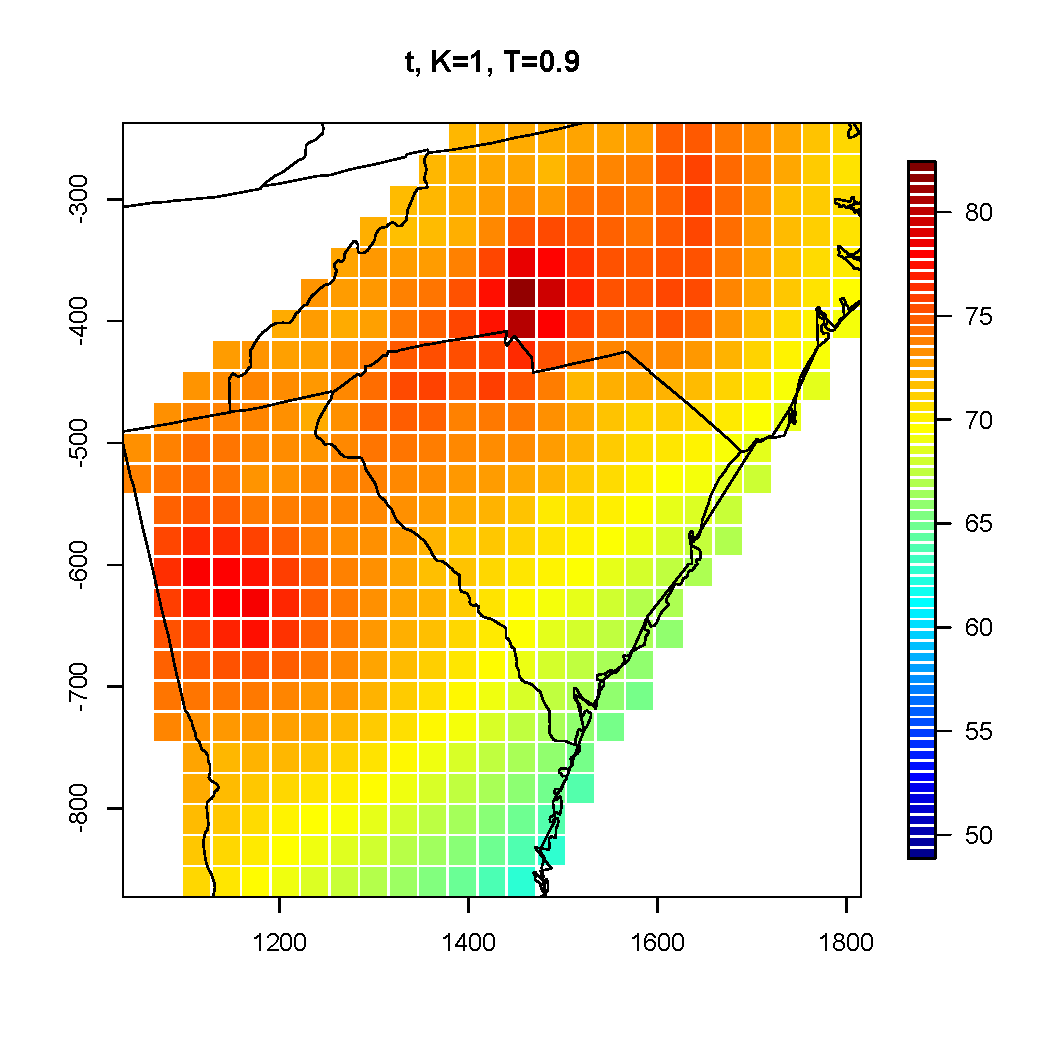
\includegraphics[width=.5\linewidth]{./plots/quantile-95-t19.pdf}
    \caption{Predicted 95th quantile using $t$ and $t$ thresholded at $T=0.9$}
\end{figure}
\end{frame}

\begin{frame}{Predicted 99th quantile}
\centering
\begin{figure}
    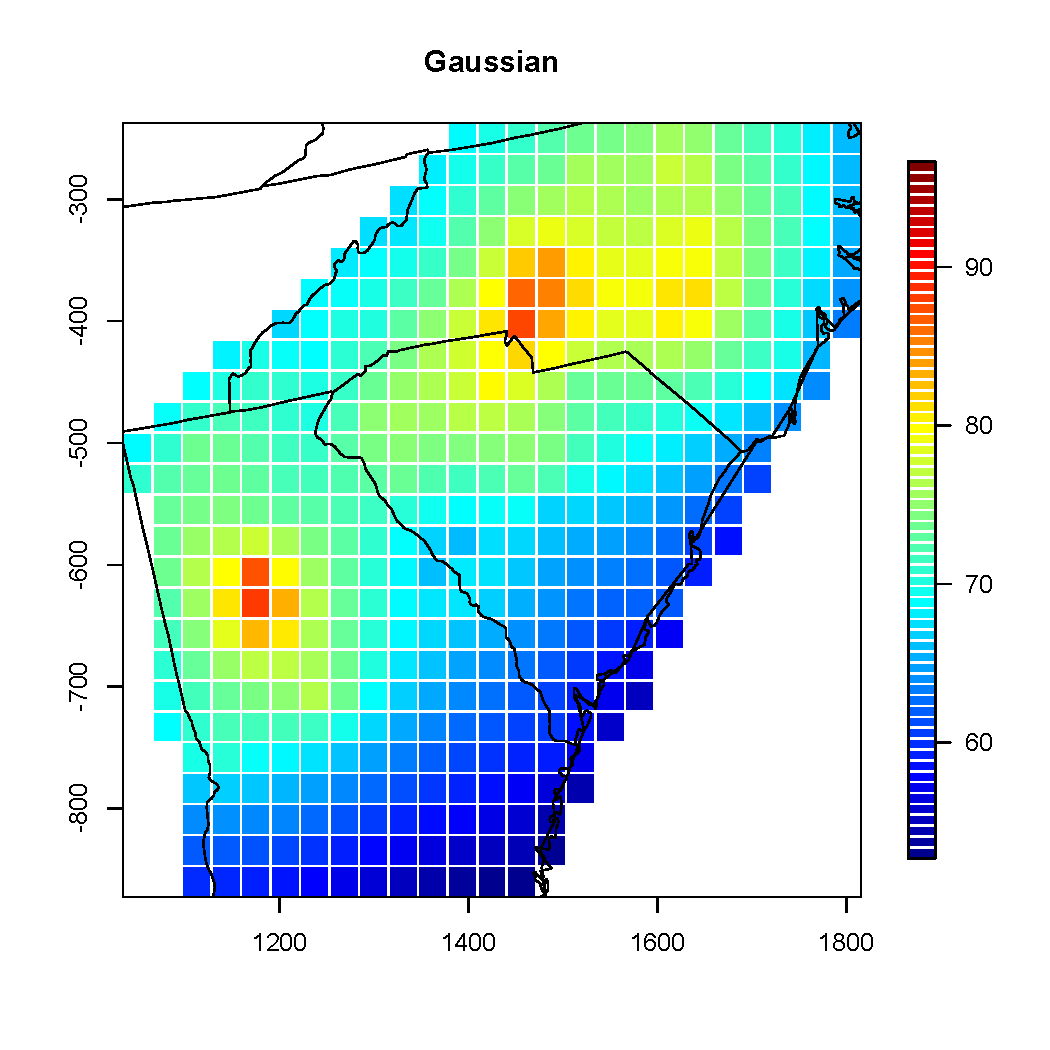
\includegraphics[width=.5\linewidth]{./plots/quantile-99-gau.pdf}
    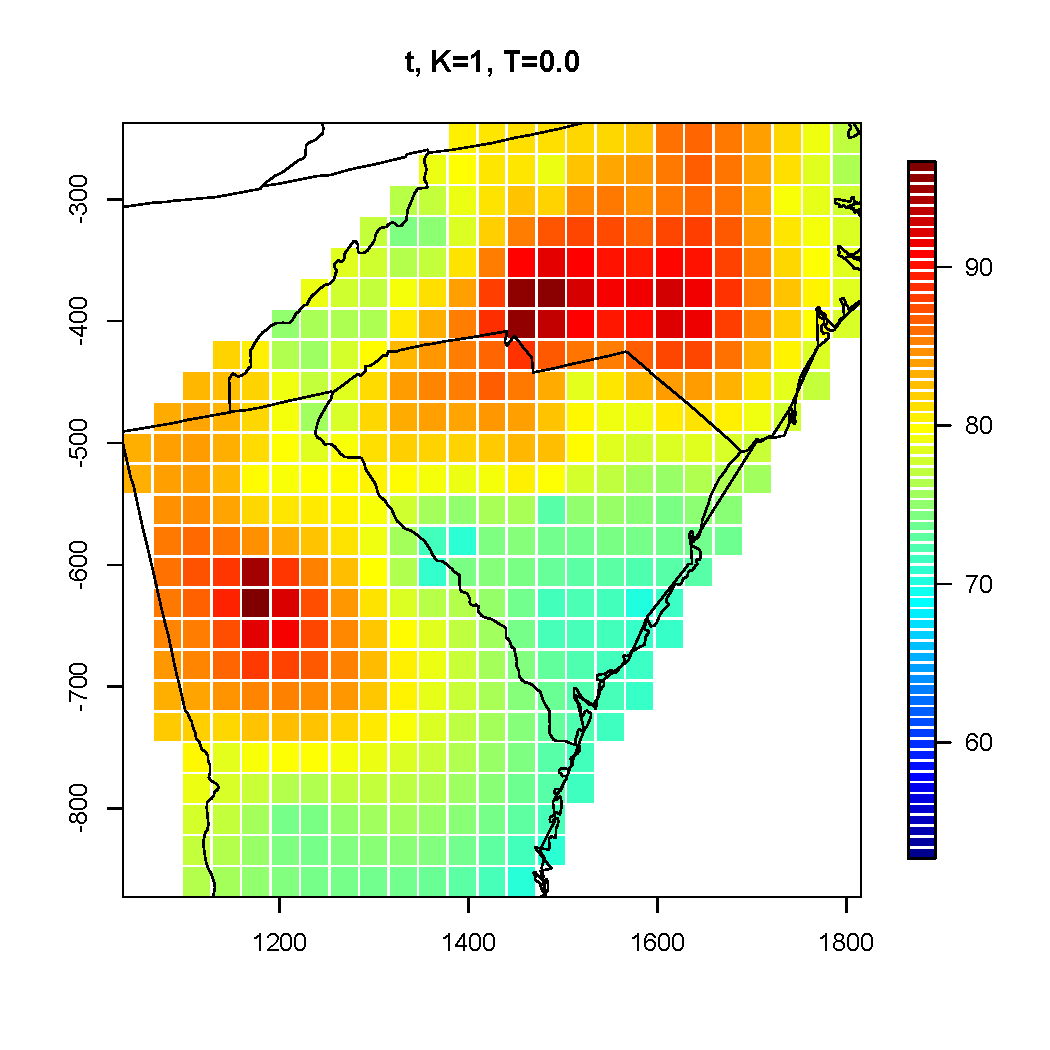
\includegraphics[width=.5\linewidth]{./plots/quantile-99-t10.pdf}
    \caption{Predicted 99th quantile using Gaussian and $t$}
\end{figure}
\end{frame}

\begin{frame}{Predicted 99th quantile}
\centering
\begin{figure}
    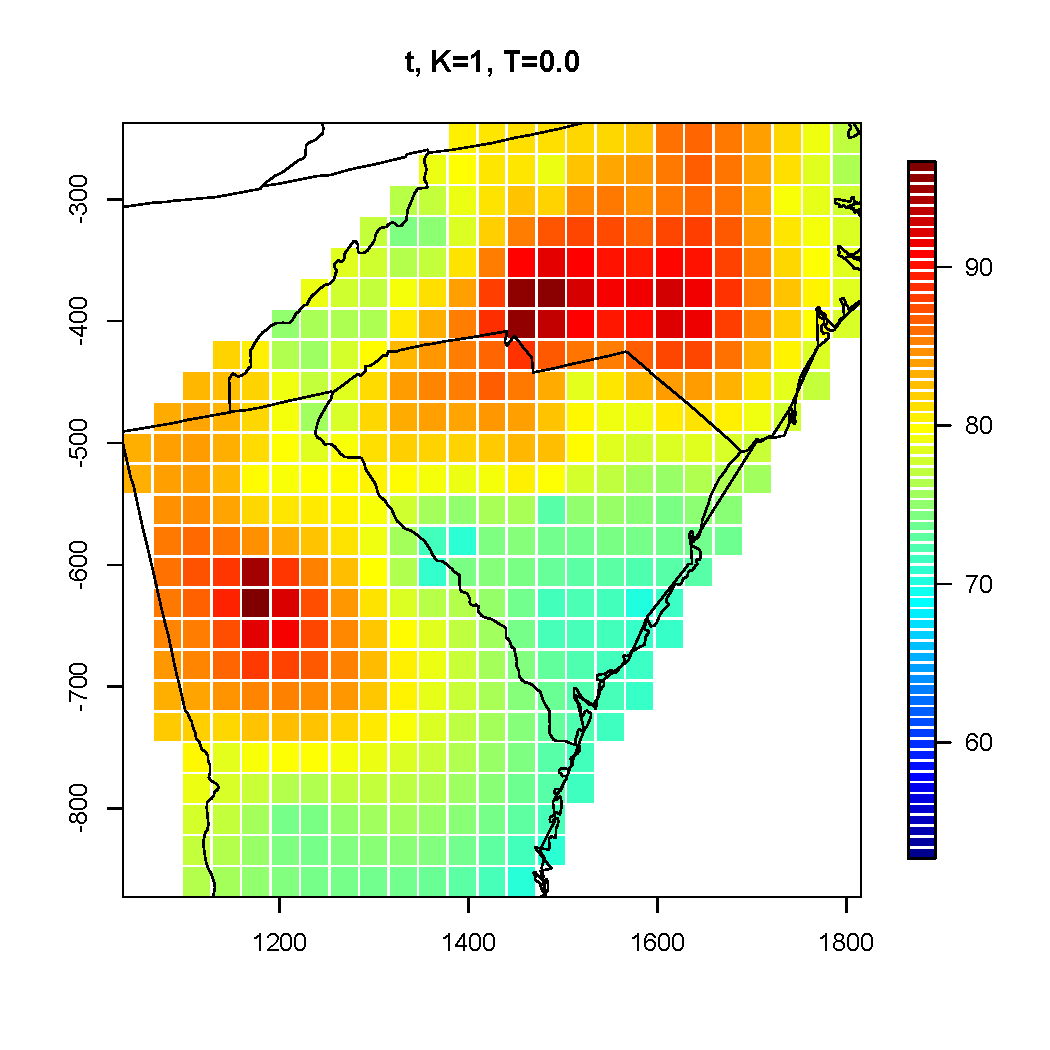
\includegraphics[width=.5\linewidth]{./plots/quantile-99-t10.pdf}
    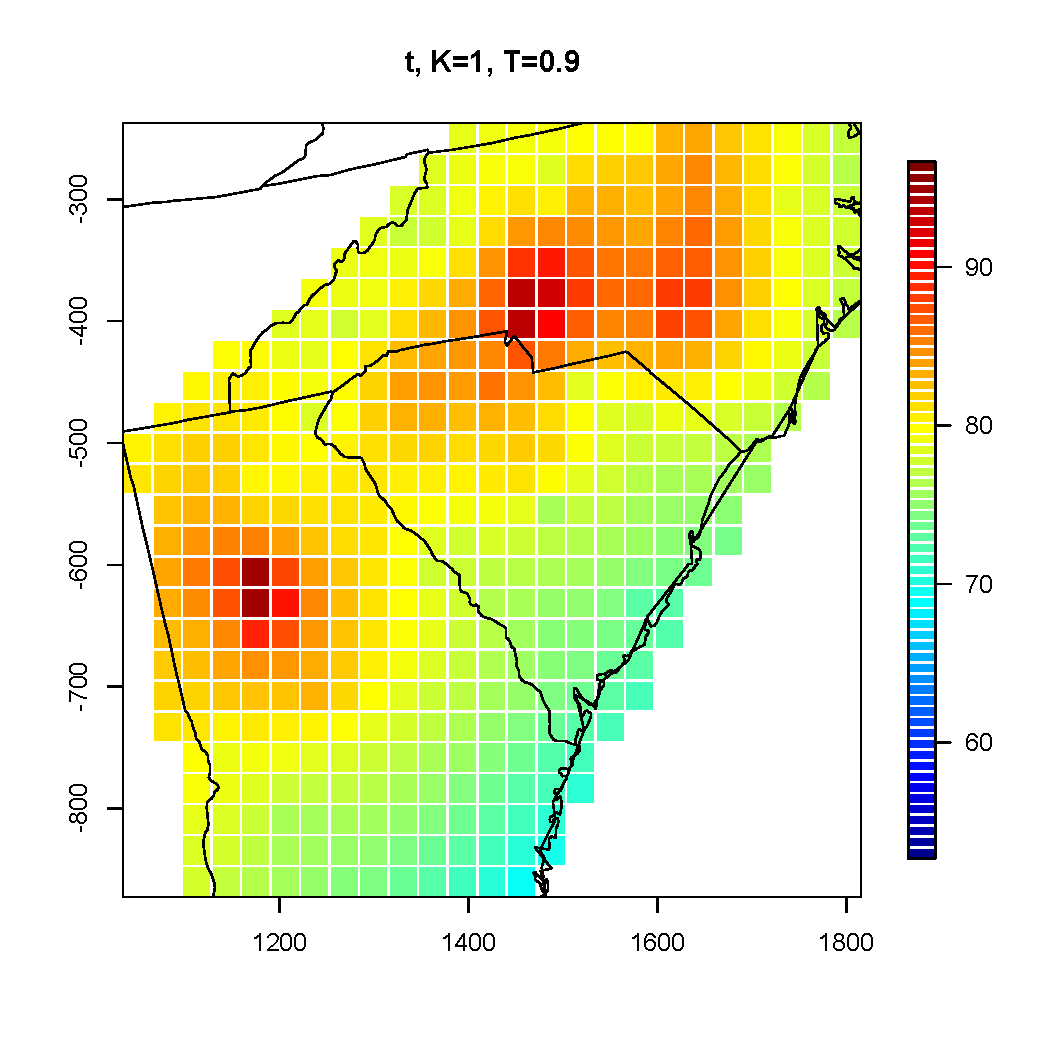
\includegraphics[width=.5\linewidth]{./plots/quantile-99-t19.pdf}
    \caption{Predicted 99th quantile using $t$ and $t$ thresholded at $T=0.9$}
\end{figure}
\end{frame}

\begin{frame}{Probability of exceedance}
\centering
\begin{figure}
    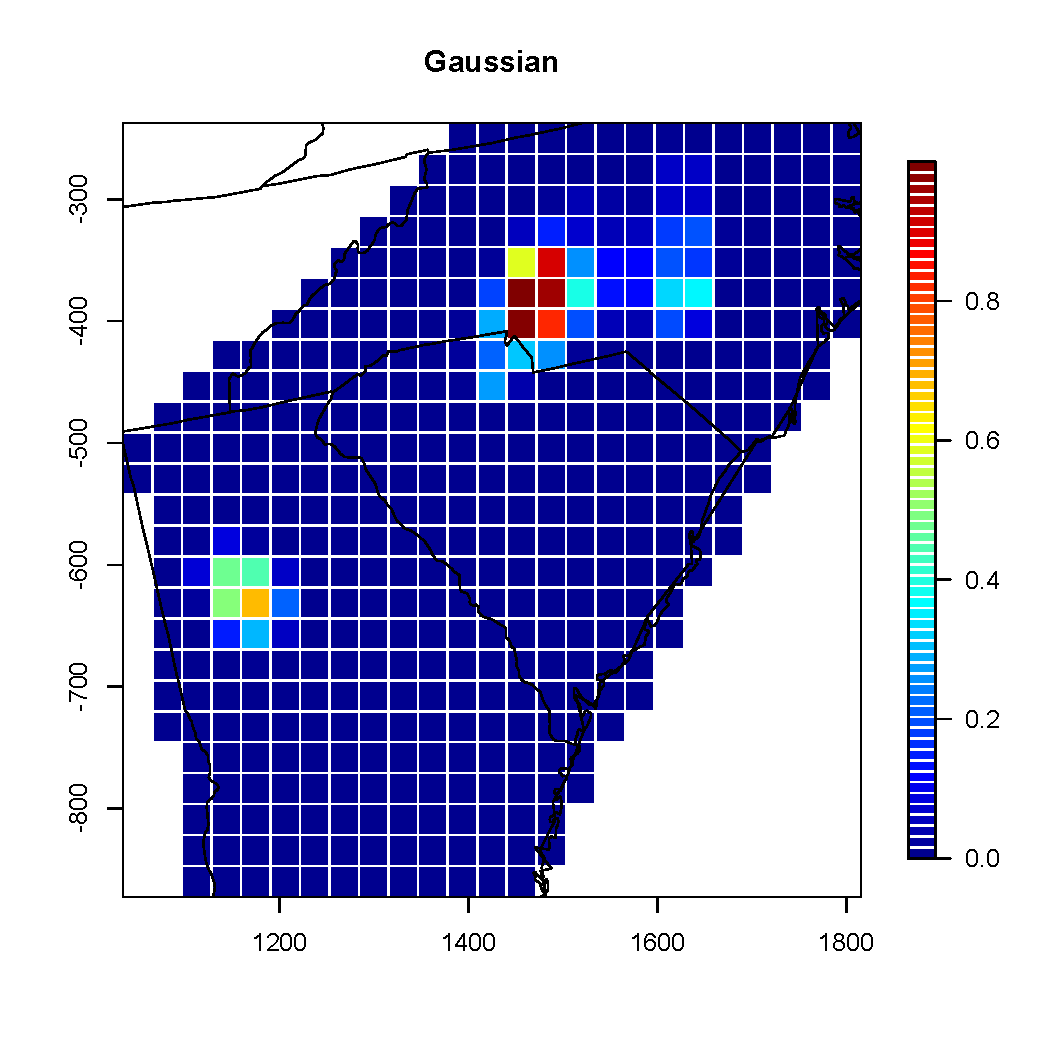
\includegraphics[width=.5\linewidth]{./plots/p-exceed-std-gau.pdf}
    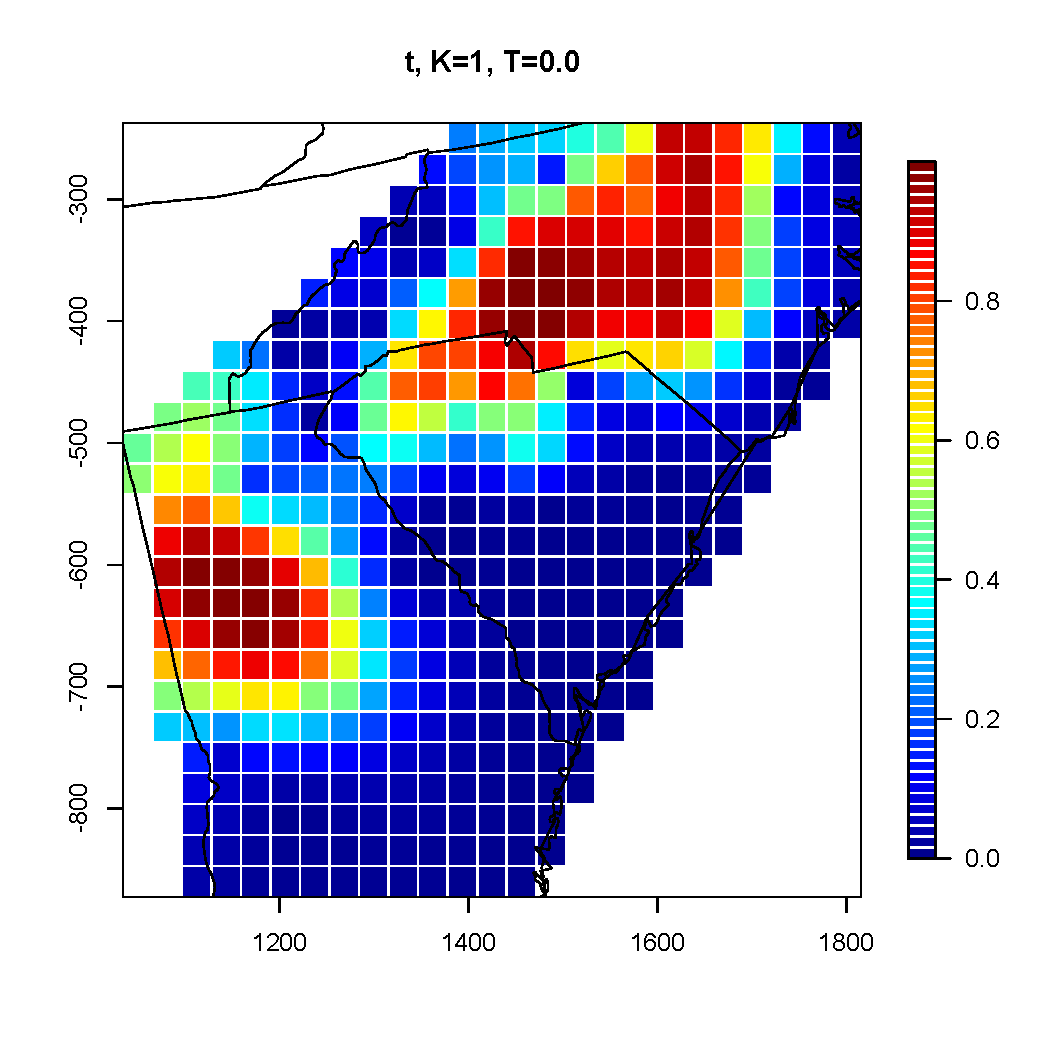
\includegraphics[width=.5\linewidth]{./plots/p-exceed-std-t10.pdf}
    \caption{Probability of exceeding the 75 ppb ozone standard using Gaussian and $t$}
\end{figure}
\end{frame}

\begin{frame}{Probability of exceedance}
\centering
\begin{figure}
    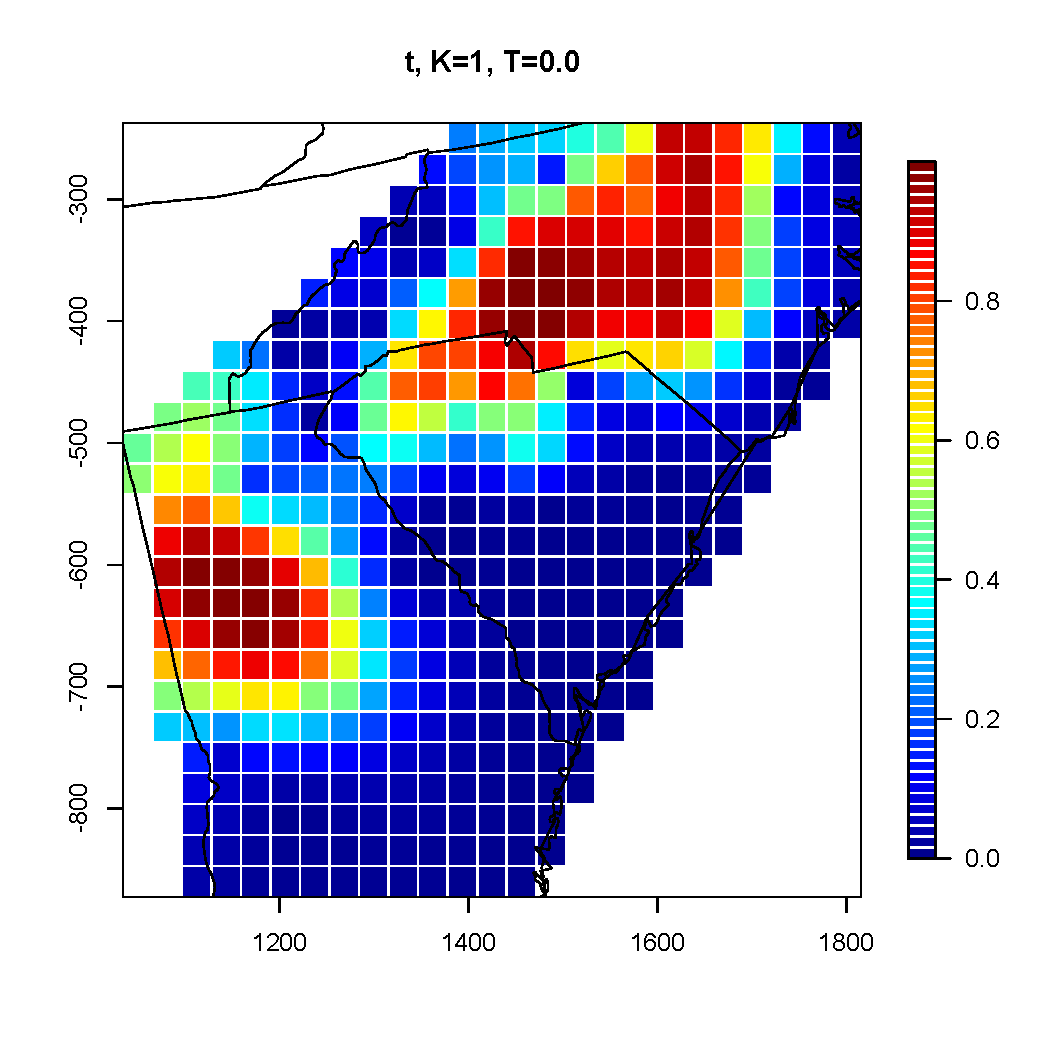
\includegraphics[width=.5\linewidth]{./plots/p-exceed-std-t10.pdf}
    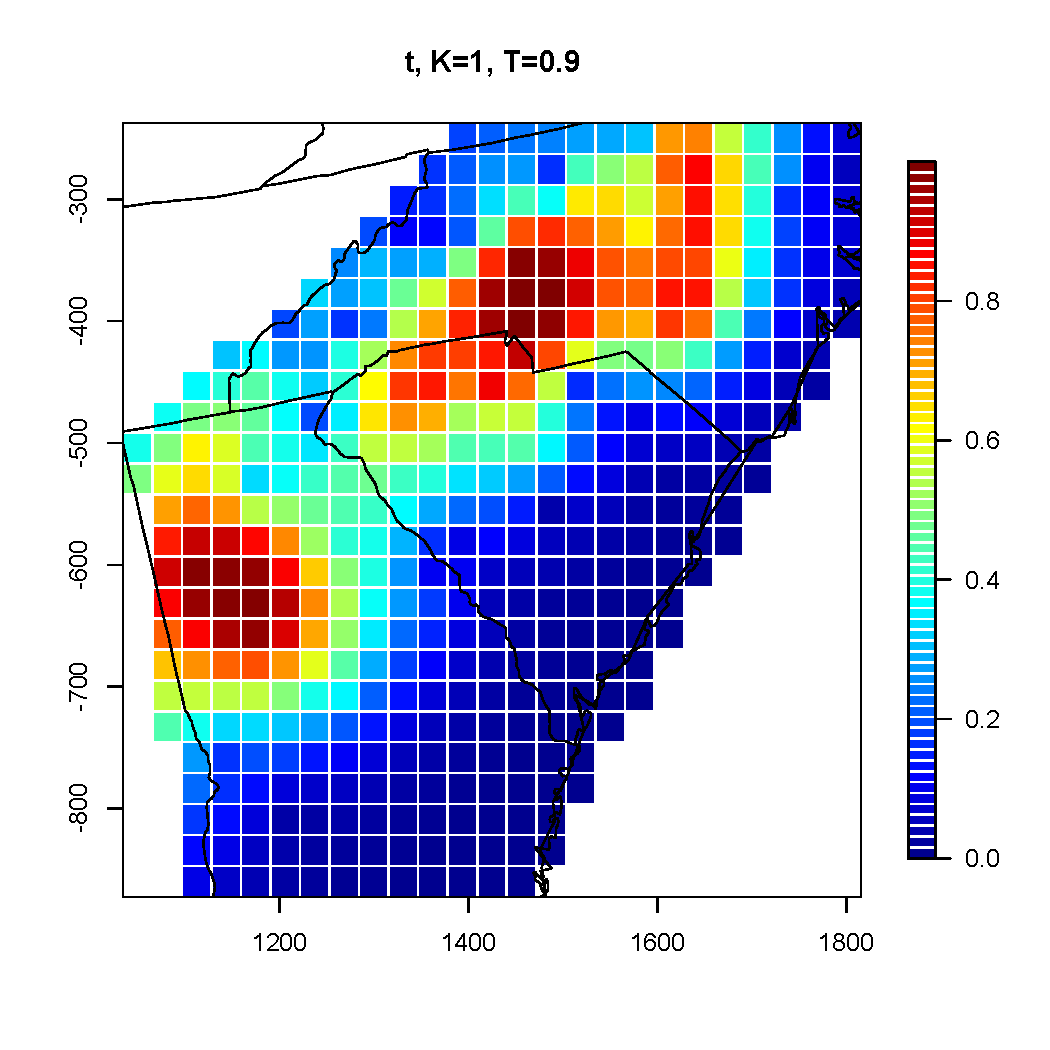
\includegraphics[width=.5\linewidth]{./plots/p-exceed-std-t19.pdf}
    \caption{Probability of exceeding the 75 ppb ozone standard using $t$ and $t$ thresholded at $T=0.9$}
\end{figure}
\end{frame}

\begin{frame}{Simulation study}
  \begin{itemize} \setlength{\itemsep}{0.5em}
    \item 6 different data settings:
    \begin{itemize}
    	\item Gaussian vs $t$ vs skew-$t$ marginal distribution
        \item $K=1$ partition vs $K=5$ partitions
    \end{itemize}
    \item Preliminary results are inconclusive
  \end{itemize}
\end{frame}

\begin{frame}{Future Work}
  \begin{itemize} \setlength{\itemsep}{0.5em}
    \item Different ways to incorporate the temporal dependence
    \begin{itemize}
    	\item Three dimensional covariance model for $v_t(\bs)$ (e.g. Huser and Davison, 2014)
    	\item Use a temporal structure for $z_t(\bs)$:
	\begin{itemize}
		\item AR(1)
		\item Moving average 
		\item Association between $\bw_{t, k}$ and $\bw_{t+1, k}$
	\end{itemize}
    \end{itemize}
     \item Comparison with extreme value analysis methods
  \end{itemize}
\end{frame}

\begin{frame}{Questions}
  \begin{itemize} \setlength{\itemsep}{0.5em}
    \item Questions?
    \item Thank you for your attention.
    \item Acknowledgment: This work was funded by EPA STAR award R835228
  \end{itemize}
\end{frame}

\begin{frame}{References}
  \begin{itemize} \setlength{\itemsep}{0.5em}
    \item Demarta, S. and McNeil, A. J. (2007) The $t$ copula and related copulas. {\it International Statistical Review}, {\bf 73}, 111--129.
    \item Huser, R. and Davison, A. C. (2014) Space-time modelling of extreme events. {\it Journal of the Royal Statistical Society: Series B (Statistical Methodology)}, {\bf 76}, 439--461.
    \item Padoan, S. A. (2011) Multivariate extreme models based on underlying skew-$t$ and skew-normal distributions. {\it Journal of Multivariate Analysis}, {\bf 102}, 977--991.
    \item Zhang, H. and El-Shaarawi, A. (2010) On spatial skew-Gaussian processes and applications. {\it Environmetrics}, {\bf 21}, 33--47.
  \end{itemize}
\end{frame}

\end{document}